\documentclass{article}

% these packages let you do math
\usepackage{amsmath}
\usepackage{amssymb}

% we need these packages for fancy R tables
\usepackage{booktabs}
\usepackage{float}
\usepackage{colortbl}
\usepackage{xcolor}

% these packages play with the spacing/margins of the document. Uncomment the commands on lines 16 and 17 to see what they do.

\usepackage{setspace}
\usepackage{geometry}

%\doublespacing
%\geometry{margin=1.5in}

% this package helps us with including images. Setting the graphics path makes it easier to refer to things in the \includegraphics command.
\usepackage{graphicx}
\graphicspath{ {../figures/} }

% make some hyperlinks using the \href command
\usepackage{hyperref}
\hypersetup{
    colorlinks=true,
    linkcolor=black,
    urlcolor=blue
}

% set the author, title, and date of the document. \maketitle adds it to the document.
\author{Liam Crawley}
\title{Incarcerations by Race and Gender using NLSY97}
\date{Sping 2022}

\begin{document}
\maketitle

\section{Analysis}

Using data from the NLSY 1997, which is a longitudinal study beginning
in 1997 and continued through 2019, we looked at incarcerations
by race and gender in 2002. Figure 1 visualizes the mean number of incarcerations
by race in 2002, color coded by gender. We see Black Males account for the largest proportion,
followed by Hispanic Males. When Mixed Race Females and Non-Blake, Non-Hispanic males 
are included with the aformentioned groups, they make up about $90\%$ of all incarcerations
in 2002 for this given sample. 
    
Table 1 is a more specific breakdown of the proportions
shown by the bar graph. It is worth noting that the proportion of Mixed Race male incarcerations
is $0.00$, which is incorrect I believe and was caused by an error summing across the data. Mixed 
Race males should account for about $4\%$ of overall incarcerations in 2002 within this sample.
Table 2 shows the regression output from a linear model using incarcerations in 2002 as the dependent
variable. We find all coefficients significant at the $5\%$ level. Holding
race constant, being male is associated with a $19.4\%$ increase in incarceration rate.
\section{Figures and Tables}

\begin{figure}[H]
    \caption{Mean Number of Incarcerations in 2002 by Race and Gender}
    \begin{center}
        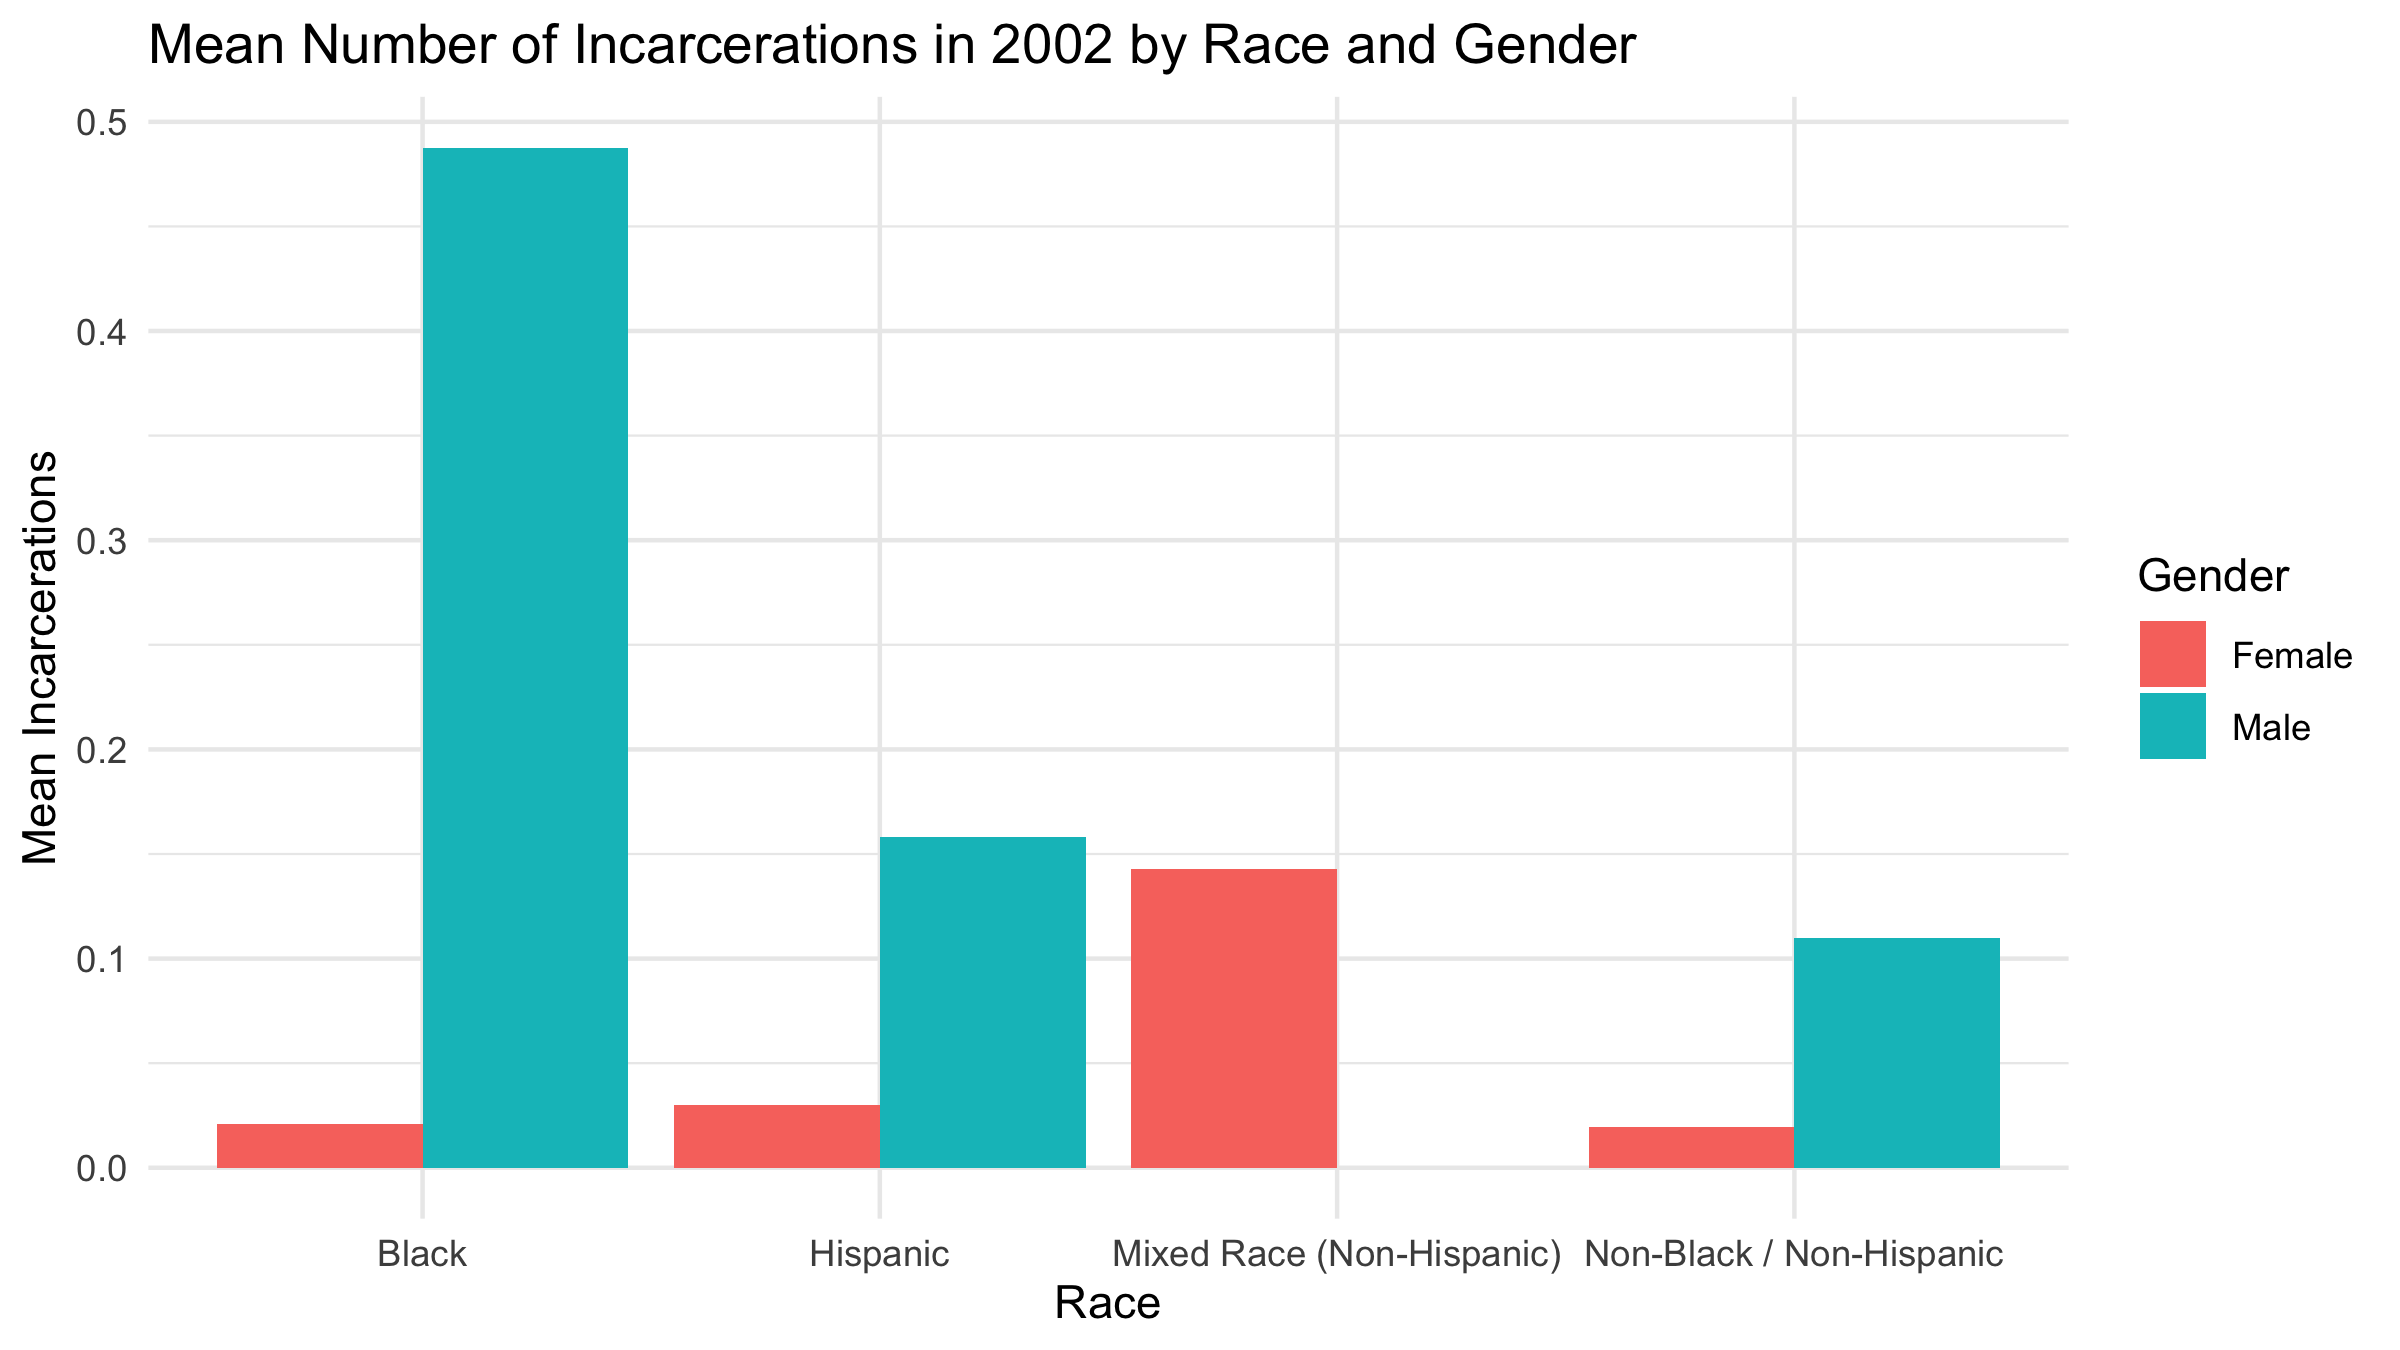
\includegraphics[width=.85\textwidth]{incarcerations_by_racegender.png}
    \end{center}
\end{figure}


\begin{table}[H]

\caption{\label{tab:tab:summarystats}Mean incarcerations in 2002 by Race and Gender}
\centering
\begin{tabular}[t]{lrrrr}
\toprule
Gender & Black & Hispanic & Mixed Race Non Hispanic & Non Black Non Hispanic\\
\midrule
\cellcolor{gray!6}{Female} & \cellcolor{gray!6}{0.0211268} & \cellcolor{gray!6}{0.0298013} & \cellcolor{gray!6}{0.1428571} & \cellcolor{gray!6}{0.0193192}\\
Male & 0.4876712 & 0.1579509 & 0.0000000 & 0.1099476\\
\bottomrule
\end{tabular}
\end{table}



% Table created by stargazer v.5.2.2 by Marek Hlavac, Harvard University. E-mail: hlavac at fas.harvard.edu
% Date and time: Wed, Feb 16, 2022 - 09:49:29
\begin{table}[!htbp] \centering 
  \caption{Regression Output. Omitted category is Black Females.} 
  \label{tab:regression} 
\begin{tabular}{@{\extracolsep{5pt}}lc} 
\\[-1.8ex]\hline 
\hline \\[-1.8ex] 
 & \multicolumn{1}{c}{\textit{Dependent variable:}} \\ 
\cline{2-2} 
\\[-1.8ex] & Incarcerations in 2002 \\ 
\hline \\[-1.8ex] 
 Hispanic & $-$0.159$^{***}$ \\ 
  & (0.038) \\ 
  & \\ 
 Mixed Race (Non-Hispanic) & $-$0.174$^{**}$ \\ 
  & (0.083) \\ 
  & \\ 
 Non-Black / Non-Hispanic & $-$0.189$^{***}$ \\ 
  & (0.035) \\ 
  & \\ 
 Male & 0.194$^{***}$ \\ 
  & (0.022) \\ 
  & \\ 
 Constant & 0.155$^{***}$ \\ 
  & (0.026) \\ 
  & \\ 
\hline \\[-1.8ex] 
Observations & 8,621 \\ 
R$^{2}$ & 0.015 \\ 
Adjusted R$^{2}$ & 0.014 \\ 
Residual Std. Error & 1.019 (df = 8616) \\ 
F Statistic & 32.033$^{***}$ (df = 4; 8616) \\ 
\hline 
\hline \\[-1.8ex] 
\textit{Note:}  & \multicolumn{1}{r}{$^{*}$p$<$0.1; $^{**}$p$<$0.05; $^{***}$p$<$0.01} \\ 
\end{tabular} 
\end{table} 





\end{document}
